\documentclass[11pt]{article}

% ---------- Page geometry ----------
\usepackage[letterpaper,margin=1in]{geometry}
\usepackage[utf8]{inputenc}
\usepackage[T1]{fontenc}
\usepackage{textcomp}
\usepackage{mathptmx} % Times-like text and math
\usepackage{microtype}
\usepackage{setspace}
\setstretch{1.15}

% ---------- Math / symbols ----------
\usepackage{amsmath,amssymb}

% ---------- Graphics / tables ----------
\usepackage{graphicx}
\usepackage{booktabs}
\usepackage{array}
\usepackage{multirow}
\usepackage{caption}
\captionsetup{font=small,labelfont=bf,justification=justified}

% ---------- References ----------
\usepackage[authoryear,round]{natbib}
\bibliographystyle{apalike}

% ---------- Links ----------
\usepackage[colorlinks=true,citecolor=black,linkcolor=black,urlcolor=black]{hyperref}

% ---------- Title spacing ----------
\usepackage{titlesec}
\titlespacing*{\section}{0pt}{14pt}{6pt}
\titlespacing*{\subsection}{0pt}{10pt}{4pt}

\title{\bfseries Does Size Generalization Imply Disruption Robustness?\\
A Pre-Registered Study of GNN--PPO Scheduling Policies for the\\
Dynamic Flexible Job-Shop Problem}

\author{
  Joseph Sanchez$^{1,2,\ast}$ \\[4pt]
  \small $^{1}$Department of Industrial Engineering, Universidad de los Andes, Bogot\'a, Colombia \\
  \small $^{2}$Corporaci\'on Universitaria Minuto de Dios (UNIMINUTO), Bogot\'a, Colombia \\[4pt]
  \small $^{\ast}$Corresponding author. E-mail: \texttt{jj.sancheza1@uniandes.edu.co} \\
  \small ORCID: 0009-0007-2008-823X
}
\date{}

% ---------- Convenience macros ----------
\newcommand{\Cmax}{C_{\max}}
\newcommand{\RPD}{\mathrm{RPD}}
\newcommand{\RI}{\mathrm{RI}}

\begin{document}

\maketitle
\thispagestyle{empty}

\begin{abstract}
\noindent
Graph neural network (GNN) policies trained with deep reinforcement learning (DRL) have been shown to generalize to job-shop instances larger than those seen during training and, separately, to be trainable for robustness against a single type of stochastic disruption. Whether these two properties---size generalization and multi-disruption robustness---co-emerge in the same policy has not previously been tested jointly under a statistically rigorous, pre-registered protocol. This study trains a relational graph-isomorphism-network (GIN) encoder with a proximal policy optimization (PPO) policy for the dynamic, stochastic flexible job-shop problem (FJSP) and pre-registers five hypotheses (H1--H5), with decision rules frozen before any experiment was run, evaluated against nine priority dispatching rules (PDR), a genetic algorithm (GA), and an exact constraint-programming solver (CP-SAT) across the Fisher--Thompson, Lawrence, and Brandimarte benchmark families. Four of five hypotheses are rejected. The policy does not match the best dispatching rule on static instances (H1: mean relative percentage deviation [RPD] 24.82\% versus 18.96\%, $N=43$, $p=4.03\times10^{-5}$); it is not robust under nine disruption regimes spanning machine breakdowns, stochastic processing times, and dynamic arrivals (H3: $p<1.7\times10^{-11}$ in all nine regimes); and augmenting the reward with a disruption-aware instability penalty fails to improve robustness without collapsing nominal performance (H4: nominal RPD increases by 46.6 to 106.0 percentage points). Decision latency is one to two orders of magnitude below the solver's on large, hard instances, but does not clear the strict pre-registered threshold on every instance (H5). Size generalization, by contrast, is accepted (H2): across four size tiers ($1.5\times$--$3.0\times$ the training size), the policy's rank among ten methods is never significantly worse than the best dispatching rule's, even though its absolute optimality gap remains uncompetitive. We argue that this pattern---architectural transfer of rank without transfer of competitiveness, and no automatic transfer of robustness---is itself the study's central, defensible contribution: size generalization and multi-disruption robustness are separable properties of GNN--PPO scheduling policies, not a package deal, diagnosed here for the first time under a pre-registered, statistically powered, jointly tested protocol, with a concrete, actionable mechanism identified for every rejection.

\medskip
\noindent\textbf{Keywords:} Deep reinforcement learning; Graph neural networks; Flexible job-shop scheduling; Dynamic and stochastic scheduling; Robustness; Size generalization; Pre-registration; Proximal policy optimization
\end{abstract}

\newpage
\setcounter{page}{1}

% ============================================================================
\section{Introduction}
% ============================================================================

The fourth industrial revolution has turned discrete manufacturing into a data-intensive, interconnected system of sensors, programmable controllers, and cyber-physical production platforms. Within this environment, production scheduling---the assignment of operations to machines over time---remains one of the most consequential and, at the same time, one of the hardest decision functions to automate robustly on a real shop floor \citep{pinedo2022}. The flexible job-shop scheduling problem (FJSP) generalizes the classical job-shop scheduling problem (JSSP) by allowing each operation to be processed on more than one candidate machine, adding a routing decision on top of the traditional sequencing decision \citep{brandimarte1993}. This flexibility is operationally desirable---it improves resource utilization and operational resilience---but it substantially increases combinatorial complexity: the JSSP is already strongly NP-hard for three or more machines \citep{garey1976}, and the FJSP contains it as a special case.

The motivation for this study, however, is not combinatorial hardness on its own, but a more specific and industrially relevant gap: real shop floors are neither static nor deterministic. Machines break down, processing times deviate from nominal estimates, and jobs arrive without complete advance notice. Exact methods---constraint programming, mixed-integer programming---guarantee optimality only at a computational cost that grows prohibitively with instance size; priority dispatching rules (PDR) and metaheuristics trade solution quality for speed; and neither family adapts natively to events that occur \emph{during} schedule execution \citep{pinedo2022,graham1979}.

In recent years, deep reinforcement learning \citep{sutton2018} combined with graph neural networks has emerged as an alternative paradigm: rather than resolving each instance from scratch, a policy is trained once and applied, in amortized fashion, to the partial state of a shop represented as a graph. \citet{zhang2020l2d}'s L2D showed that a graph-isomorphism-network (GIN) encoder paired with a proximal policy optimization (PPO) policy \citep{schulman2017ppo}, trained on small instances, can outperform classical dispatching rules and approach the solution quality of an exact solver on static job-shop instances of increasing size, with decision times orders of magnitude below those of exact search. Subsequent work extended this paradigm to the FJSP through heterogeneous graph representations that capture both operation--operation and operation--machine relations \citep{song2023,lei2022}.

However, a systematic review of the 2015--2026 literature (Section~\ref{sec:litrev}) shows that the large majority of this line of work evaluates policies under static, deterministic conditions, or introduces at most one type of disruption at a time---machine breakdowns, or dynamic arrivals, or stochastic processing times, but rarely more than one simultaneously---and never jointly with a size-generalization claim tested under a common statistical protocol. Two recent threads come closest, each covering a single axis: \citet{smit2025spmdan} demonstrate strong size generalization under a single source of uncertainty (stochastic processing times); \citet{lassoued2026} combine two disruption types (breakdowns and arrivals) but report no size-transfer experiment and use no graph encoder at all. To our knowledge, no published work tests both axes---size generalization and multi-disruption robustness---jointly, under a pre-registered, statistically powered protocol. This is the gap the present study addresses.

We train a relational-GIN, PPO-based policy for the dynamic and stochastic FJSP and pre-register five hypotheses---H1 (static competitiveness), H2 (size generalization), H3 (robustness under disruption), H4 (whether a disruption-aware reward term improves robustness without a large nominal-performance cost), and H5 (decision-latency advantage)---with decision rules frozen before any experiment was run, following the anti-HARKing (hypothesizing after results are known) discipline increasingly expected in empirical machine-learning research. Our central contribution is not a positive result: four of the five hypotheses are rejected. It is a diagnosed, statistically rigorous characterization of exactly where, and why, the joint objective of generalization and robustness fails. Specifically, this study contributes:

\begin{enumerate}
  \item[(i)] the first, to our knowledge, jointly pre-registered test of size generalization and multi-type disruption robustness for a GNN--PPO scheduling policy, with accept/reject rules frozen before any result existed;
  \item[(ii)] a statistically powered comparison---Wilcoxon signed-rank and Friedman--Nemenyi tests with reported effect sizes---against nine dispatching rules, a tuned genetic algorithm, and an exact solver under a matched time budget, a combination rarely reported jointly in the literature reviewed;
  \item[(iii)] a root-cause diagnosis for every rejected hypothesis rather than an unexplained negative result, including a concrete, transferable mechanism---domain-randomized training without nominal-episode exposure---for why disruption-aware reward shaping collapses static performance; and
  \item[(iv)] direct empirical evidence that architectural size-invariance transfers rank-relative competitiveness even from a weak base policy, supporting a multiplicative reading of permutation-invariance-based GNN generalization theory \citep{xu2019gin}.
\end{enumerate}

The remainder of this article is organized as follows. Section~\ref{sec:litrev} reviews the related literature and formalizes the research gap. Section~\ref{sec:methods} details the problem formulation, policy architecture, baselines, and pre-registered experimental protocol. Section~\ref{sec:results} reports the results for H1--H5. Section~\ref{sec:discussion} discusses the findings in relation to prior work, their theoretical and practical implications, and the study's limitations. Section~\ref{sec:conclusion} concludes.

% ============================================================================
\section{Literature Review}
\label{sec:litrev}
% ============================================================================

\subsection{Deep reinforcement learning and graph neural networks for job-shop scheduling (2020--2023)}

The paradigm of solving combinatorial problems through learned policies, rather than hand-designed heuristics, originates outside scheduling proper, with sequence-to-sequence pointer networks for the traveling-salesman problem \citep{vinyals2015pointer} and attention-based construction heuristics trained with policy gradients \citep{kool2019attention,kwon2020pomo}. The foundational application to job-shop scheduling is \citet{zhang2020l2d}'s L2D, which pairs a disjunctive-graph representation with a GIN encoder \citep{xu2019gin} and a PPO policy that decides, at each decision epoch, which operation to dispatch. L2D reports optimality gaps of 13.6--29.2\% against OR-Tools on generated and Taillard \citep{taillard1993} instances, outperforming classical dispatching rules on 87.5--92\% of evaluated instances, and---critically for the present study---demonstrates out-of-distribution size generalization: a policy trained on $20\times20$/$30\times20$ instances retains a 9.4\% gap when evaluated zero-shot on $100\times20$ instances, far below the best dispatching rule's 33.7--54.9\% gap at that size. \citet{park2021} independently formalize a similar representation-and-policy-learning approach, reporting a 14.7\% mean relative error against a battery of classical and neural baselines. Both works are restricted to static, deterministic JSSP with fixed machine routing.

Extending this paradigm to the FJSP requires representing two distinct entity types---operations and machines---with distinct relations between them. \citet{song2023} propose a heterogeneous graph that augments the disjunctive graph with explicit machine nodes processed via heterogeneous attention layers, paired with a PPO policy; \citet{lei2022} propose a multi-action, dual-PPO scheme over a disjunctive-graph encoding, evaluated on the Brandimarte \citep{brandimarte1993} benchmark. Both report qualitative superiority over dispatching-rule baselines, although the exact figures could not be independently re-verified from open-access sources at the time of this review. This period also produced open-source infrastructure---Gymnasium-compatible environments \citep{tassel2021}, reusable experiment frameworks \citep{waubert2023schlably}, and unified benchmarks \citep{reijnen2023benchmark}---that makes independent reproduction and extension of this line of work tractable outside dedicated laboratories, including the pipeline underlying the present study.

\subsection{Size generalization and the homogeneous--heterogeneous architecture spectrum}

The theoretical basis for size generalization in GNN-based policies rests on permutation invariance and a parameter count that is independent of instance size: a sufficiently expressive message-passing scheme distinguishes graph structures up to the Weisfeiler--Lehman test, and a GIN encoder attains this bound \citep{xu2019gin}; related message-passing architectures include graph convolutional networks \citep{kipf2017gcn}, GraphSAGE \citep{hamilton2017graphsage}, and graph attention networks \citep{velickovic2018gat}. \citet{smit2024survey}'s survey of GNN applications to job-shop and flexible job-shop scheduling offers the most current taxonomic map of this design space and is adopted here as a classification reference. Architecturally, the literature spans a spectrum rather than a binary choice: at one end, L2D's fully homogeneous graph aggregates every edge type with a single set of weights; at the other, \citet{song2023}'s and related heterogeneous designs assign distinct transformations and attention mechanisms to each node and edge type. A third position, of very recent origin, directly challenges the near-universal 2022--2024 assumption that heterogeneity is a precondition for scalability: \citet{hoss2026} propose a feature-based homogenization that projects distinct node roles into a shared latent space, reporting linear complexity on industrial-scale instances without sacrificing performance. This debate is directly relevant to the architectural choice made in Section~\ref{sec:architecture}.

On the generalization-under-uncertainty axis specifically, \citet{smit2025spmdan}'s SPM-DAN extends a heterogeneous deep-attention-network architecture with a scenario-processing module that aggregates, via attention, multiple sampled realizations of stochastic processing times; trained on $20\times10$ instances, it maintains a $-7.10\%$ to $-7.07\%$ gap against CP-SAT when transferred, without retraining, to $30\times10$/$40\times10$ instances---a markedly stronger absolute generalization result than reported in Section~\ref{sec:h2} below, obtained under a single uncertainty source with an architecture purpose-built for it. \citet{infantes2024wheatley}'s Wheatley similarly targets generalization and scalability for JSSP with uncertain durations, minimizing expected rather than deterministic makespan. Neither work addresses multiple simultaneous disruption types.

\subsection{Robustness to disruption in dynamic and stochastic scheduling}

Beyond the static-generalization literature, work on dynamic scheduling with reinforcement learning can be organized by how uncertainty enters the Markov decision process: \emph{purely reactive} schemes, where the agent simply re-decides at each new epoch with no explicit anticipation mechanism; \emph{risk-aware} schemes, where the training objective incorporates a tail measure of the outcome distribution (e.g., SPM-DAN's value-at-risk surrogate or Wheatley's expected-makespan objective) rather than the expectation alone; and \emph{anticipatory} schemes, where the agent receives explicit distributional information about future events---a direction that remains largely unresolved in the reviewed literature. \citet{lassoued2026} combine machine breakdowns (Weibull time-to-failure) and dynamic arrivals (Gamma process) over a colored-timed-Petri-net representation with a maskable-PPO policy---no graph encoder, no size-transfer experiment---reporting 1.1--3\% improvement over the best heuristic under breakdowns alone and up to 8\% under the combined regime. This is, to our knowledge, the closest prior demonstration that a policy-gradient method can outperform dispatching rules under multi-type disruption when robustness is the sole training objective, uncontested by a shared size-generalization budget---a contrast we return to in Section~\ref{sec:discussion}. On reward design specifically, \citet{zhang2024rewardshaping} propose a heterogeneous multi-agent D3QN scheme with disruption-aware reward shaping for the dynamic FJSP under stochastic transport times---the closest precedent to the instability-penalty mechanism evaluated in Section~\ref{sec:reward}---but designed and evaluated for a single disruption type in a non-GNN, non-policy-gradient architecture.

A pattern recurs across this literature: the large majority of technical works isolate a single uncertainty axis by experimental design, even where the underlying architecture could plausibly support more than one. A partial exception is \citet{lassoued2026} (breakdowns and arrivals jointly, without size generalization or a graph encoder); in a methodologically distinct paradigm, large-language-model scheduling agents have also been evaluated under multiple simultaneous event types without parametric training \citep{cao2025reflecsched}.

\subsection{An emerging, methodologically distinct paradigm: LLM-based scheduling agents}

A rapidly growing body of 2025--2026 work applies pretrained large language models (LLMs), guided by prompting, simulated rollouts, or supervised fine-tuning, directly to scheduling decisions rather than training a fixed-parameter policy by reward gradient \citep{abgaryan2025starjob,cao2025reflecsched}. Their relationship to size generalization is qualitatively different from a GNN's: rather than an architectural invariance to instance dimensions, these agents inherit generalization from large-scale language pretraining. We treat this paradigm as a point of discursive contrast in Section~\ref{sec:discussion} rather than a direct methodological competitor, since the policy evaluated here is a trained, fixed-parameter GNN--PPO model, not a prompted language-model agent.

\subsection{Research gap and hypotheses}
\label{sec:gap}

Table~\ref{tab:gap} synthesizes the gap analysis underlying this study, drawn from a systematic search of 2015--2026 literature (arXiv, Semantic Scholar, DBLP, and open-access publisher indices) using four query strings combining reinforcement-learning, graph-neural-network, job-shop/flexible-job-shop, and dynamic/stochastic/disruption terms.

\begin{table}[htbp]
\centering
\caption{Research gap synthesis: identified gaps, representative 2024--2026 evidence, and status after this review.}
\label{tab:gap}
\small
\begin{tabular}{p{3.6cm}p{5.8cm}p{4.4cm}}
\toprule
\textbf{Identified gap} & \textbf{Representative evidence} & \textbf{Status after this review} \\
\midrule
Joint test of size generalization \emph{and} multi-disruption robustness &
\citet{smit2025spmdan} and \citet{infantes2024wheatley} generalize in size under one uncertainty source; \citet{lassoued2026} combine two disruption types with no size-transfer test and no graph encoder &
Confirmed open; central axis of this study (H2 + H3/H4 jointly) \\
\addlinespace
Disruption-aware reward shaping restricted to a single event type &
\citet{zhang2024rewardshaping} design reward shaping for one disruption type in a non-GNN, multi-agent architecture &
Narrowed, not closed; H4 tests generalization to a multi-disruption regime \\
\addlinespace
Simultaneous, time-matched comparison against CP-SAT, a genetic algorithm, and PDR &
No 2024--2026 work identified in this review reports all three baseline families jointly under a matched time budget &
Confirmed open; addressed by the experimental design (Section~\ref{sec:baselines}) \\
\addlinespace
Non-parametric statistical protocol with effect sizes and critical-difference diagrams &
Not reported in any 2024--2026 work identified in this review &
Confirmed open; addressed throughout Section~\ref{sec:results} \\
\addlinespace
Assumption that a heterogeneous graph representation is necessary for size generalization &
Near-universal assumption 2022--2024; directly challenged by \citet{hoss2026} via linear-complexity homogenization &
Emerging, unsettled; informs the architectural choice in Section~\ref{sec:architecture} \\
\bottomrule
\end{tabular}
\end{table}

Across the technical works surveyed, the specific combination this study investigates---size generalization and robustness to multiple simultaneous disruption types, tested jointly and statistically on a single pre-registered policy---remains unresolved. Guided by this gap, the study tests five hypotheses: static competitiveness against the best dispatching rule (H1); generalization to instances $1.5\times$--$3.0\times$ the training size (H2); robustness, relative to dispatching rules, under nine disruption regimes spanning machine breakdowns, stochastic processing times, and dynamic arrivals (H3); whether an explicit disruption-aware reward term improves robustness without an unacceptable nominal-performance cost (H4); and whether decision latency remains far below that of an exact solver as instance size grows (H5). Section~\ref{sec:prereg} states the exact, pre-registered decision rule for each hypothesis.

% ============================================================================
\section{Materials and Methods}
\label{sec:methods}
% ============================================================================

\subsection{Problem formulation}

This study addresses the dynamic, stochastic FJSP. A set of jobs $J=\{1,\dots,n\}$ is defined, each a fixed-precedence sequence of operations $O_{j,h}$; each operation is processable on any machine in an eligible subset $M_{j,h}\subseteq M$, with machine-dependent processing time $p_{j,h,k}$. Three sources of uncertainty extend the deterministic base problem: (i) dynamic job arrivals, modeled as a Poisson process calibrated to a target utilization $\rho$; (ii) stochastic processing times, a log-normal multiplier of unit mean applied to the nominal duration; and (iii) machine breakdowns, with exponential time-to-failure and log-normal time-to-repair, parameterized by a target steady-state availability $A_k$. The environment is realized as a discrete-event simulation exposed through a Gymnasium-compatible interface (cf.\ \citealp{tassel2021}); each decision epoch corresponds to one \texttt{step()} call, with a legality mask recomputed at every step to exclude infeasible operation--machine assignments.

\subsection{Policy architecture}
\label{sec:architecture}

At decision epoch $t$, the state is represented as a heterogeneous graph $G_t = (O_t \cup M,\ E^{\mathrm{prec}} \cup E^{\mathrm{mach}} \cup E^{\mathrm{elig}})$ over operation nodes $O_t$ and machine nodes $M$, connected by three typed relations: intra-job precedence, shared-machine competition among undispatched operations, and operation--machine eligibility. We adopt a \textbf{relational GIN}---a single node type with three separate linear transformations, one per edge type, aggregated by summation before a GIN update---rather than the fully homogeneous graph of L2D \citep{zhang2020l2d} or the fully heterogeneous, attention-based graph of \citet{song2023}. This is a deliberate midpoint of the homogeneous--heterogeneous spectrum discussed in Section~\ref{sec:gap}: more expressive than a single shared adjacency, because it distinguishes the opposing semantics of each relation (a predecessor constrains, a successor is constrained, a machine competitor contests the same resource), without the parameter and computational cost of full heterogeneity---and consistent with \citet{hoss2026}'s evidence that heterogeneity is not a strict precondition for scalable generalization. Sum aggregation, rather than mean or max, is used throughout, following the expressiveness argument of \citet{xu2019gin}---a property required for the policy to distinguish, for instance, a lightly loaded machine from a heavily loaded one.

Message passing at layer $l$ for an operation node $v$ and a machine node $k$ is given by:
\begin{align}
h_v^{(l)} &= \mathrm{MLP}_O^{(l)}\left((1{+}\epsilon^{(l)})h_v^{(l-1)} + W_{\mathrm{pred}}\!\!\sum_{u\to v}\!h_u^{(l-1)} + W_{\mathrm{succ}}\!\!\sum_{v\to u}\!h_u^{(l-1)} + W_{\mathrm{mach}}\!\!\sum_{u\sim v}\!h_u^{(l-1)} + W_{\mathrm{elig}}\,h_{m(v)}^{(l-1)}\right) \label{eq:gin-op}\\[4pt]
h_k^{(l)} &= \mathrm{MLP}_M^{(l)}\left((1{+}\epsilon_M^{(l)})h_k^{(l-1)} + W_{\mathrm{cand}}\!\!\!\sum_{v:\,m(v)=k}\!\!\!h_v^{(l-1)}\right) \label{eq:gin-mach}
\end{align}
where $h$ denotes a node embedding, $\epsilon^{(l)}$ and $\epsilon_M^{(l)}$ are learnable GIN self-weighting scalars, and $W_{\mathrm{pred}}, W_{\mathrm{succ}}, W_{\mathrm{mach}}, W_{\mathrm{elig}}, W_{\mathrm{cand}}$ are relation-specific linear transformations.

A per-node actor head, shared across all operation embeddings, produces one logit per candidate operation regardless of instance size, softmax-normalized over legal actions only, with the mask applied before log-probability computation rather than as a reward penalty \citep{huang2022masking}. The actor's parameter count is, by construction, independent of the number of operations $N$---the architectural property underlying the size-generalization hypothesis (H2). The critic consumes a mean-pooled graph embedding. Training uses MaskablePPO \citep{raffin2021sb3} with a clipped surrogate objective and generalized advantage estimation \citep{schulman2016gae}, with discount factor $\gamma=1$, justified by the reward's telescoping-sum structure described next.

\subsection{Disruption-aware reward}
\label{sec:reward}

The base reward is dense and potential-based:
\begin{equation}
r_t = \big(H(s_t) - H(s_{t+1})\big) \times \text{reward\_scale},
\end{equation}
where $H(s)$ is a state-dependent lower-bound estimate of the makespan (an optimistic job-chain propagation that ignores machine contention on undispatched operations), guaranteeing $r_t \le 0$ and a telescoping return $\sum_t r_t = (H(s_0) - \Cmax)\times\text{reward\_scale}$; maximizing undiscounted return is therefore exactly equivalent to minimizing makespan \citep{ng1999shaping}. To test H4, this reward is extended with an instability penalty:
\begin{equation}
r_t = (LB_{t-1} - LB_t)\times\text{reward\_scale} - \kappa\cdot\Delta_{\mathrm{inest}}\times\text{reward\_scale},
\end{equation}
where $\Delta_{\mathrm{inest}}$ is the deviation from previously planned start times induced by re-planning after a disruption event, and $\kappa\in\{0,0.5,1.0\}$; $\kappa=0$ recovers the base reward exactly (verified by unit test).

\subsection{Baseline methods}
\label{sec:baselines}

Nine priority dispatching rules (PDR) are evaluated: shortest processing time (SPT), longest processing time (LPT), most work remaining (MWKR), least work remaining (LWKR), most operations remaining (MOR), least operations remaining (LOR), first-in-first-out (FIFO), earliest due date (EDD), and critical ratio (CR); the last two require synthesized due dates via the total-work-content rule, $d_j = r_j + 1.5\sum_h p_{j,h}$, since the benchmark families used carry no published due dates. A genetic algorithm (permutation-with-repetition encoding, precedence-order crossover, swap mutation, tournament selection with elitism, population size 80 scaled down for larger instances, and a 5\% random-immigrant rate against premature convergence) and CP-SAT \citep{perron2023cpsat}, Google OR-Tools' constraint-programming solver, serve as the metaheuristic and exact/near-exact references. All methods except the PDRs, which are effectively instantaneous, operate under a wall-clock budget matched to CP-SAT's (60 seconds) for a fair comparison.

\subsection{Experimental design and statistical protocol}

Evaluation spans 43 JSSP instances (Fisher--Thompson \emph{ft06/ft10/ft20}; Lawrence \emph{la01}--\emph{la40}) and two FJSP arms: a synthetic arm (the same 43 base instances extended with machine flexibility) and seven of the eight Brandimarte instances (\emph{mk06} excluded after an upstream benchmark-mirror inconsistency---15 machines instead of the published 10---was traced during instance loading). All pairwise comparisons use the exact Wilcoxon signed-rank test; joint comparisons across the ten methods (the policy plus nine PDRs) use the Friedman test with Nemenyi post-hoc analysis and critical-difference diagrams \citep{demsar2006}; effect sizes ($r = Z/\sqrt{N}$) are reported throughout.

\subsection{Pre-registration and hypotheses}
\label{sec:prereg}

Five hypotheses were pre-registered, with quantitative accept/reject rules frozen in a timestamped document before any policy-evaluation result was generated---a discipline intended to guard against hypothesizing after results are known (HARKing), and one that Table~\ref{tab:gap} shows to be largely absent from the works surveyed in Section~\ref{sec:litrev}. Table~\ref{tab:hypotheses} states each hypothesis and its exact decision rule.

\begin{table}[htbp]
\centering
\caption{Pre-registered hypotheses and frozen decision rules.}
\label{tab:hypotheses}
\small
\begin{tabular}{cp{4.6cm}p{6.4cm}}
\toprule
\textbf{Hyp.} & \textbf{Claim} & \textbf{Accept criterion (frozen before evaluation)} \\
\midrule
H1 & The policy outperforms the best PDR in mean RPD on static instances &
Wilcoxon $p<0.05$ and $\text{median}(\RPD_{\text{bestPDR}} - \RPD_{\text{RL}}) > 0$, per instance family \\
\addlinespace
H2 & RPD on $1.5\times$--$3.0\times$ larger instances stays competitive with the best PDR &
Friedman--Nemenyi: the policy's rank not significantly worse than the best PDR's, in every size tier \\
\addlinespace
H3 & Robustness index (RI) is lower than PDRs' under breakdowns, stochastic times, and arrivals &
Wilcoxon $p<0.05$ and $\text{median}(\RI_{\text{PDR}} - \RI_{\text{RL}}) > 0$, in all 9 disruption regimes (conjunctive rule) \\
\addlinespace
H4 & $\kappa>0$ reduces RI without increasing nominal RPD by more than 2 percentage points &
$\Delta \RI<0$ significant in $\ge 5/9$ regimes \textbf{and} $\Delta \RPD_{\text{nom}} < 2$pp (both required) \\
\addlinespace
H5 & Decision latency stays far below CP-SAT's as instance size grows &
$\text{median}(\text{ms/decision}_{\text{RL}}) < 1\% \times \text{median}(\text{ms/decision}_{\text{CP-SAT}})$, for every instance \\
\bottomrule
\end{tabular}
\end{table}

% ============================================================================
\section{Results}
\label{sec:results}
% ============================================================================

Table~\ref{tab:verdicts} summarizes the verdict for all five pre-registered hypotheses; Sections~\ref{sec:h1}--\ref{sec:h5} detail each in turn.

\begin{table}[htbp]
\centering
\caption{Hypothesis verdicts (all tests two-sided, $\alpha=0.05$).}
\label{tab:verdicts}
\small
\begin{tabular}{lp{3.1cm}p{5.4cm}c}
\toprule
\textbf{Hypothesis} & \textbf{Test} & \textbf{Statistic} & \textbf{Verdict} \\
\midrule
H1 (JSSP) & Wilcoxon, $N{=}43$ & $W{=}133$, $p{=}4.03{\times}10^{-5}$, $r{=}{-}0.63$ & \textbf{REJECT} \\
H1 (FJSP synthetic) & Wilcoxon, $N{=}43$ & $W{=}0$, $p{=}1.12{\times}10^{-8}$, $r{=}{-}0.87$ & \textbf{REJECT} \\
H1 (FJSP Brandimarte) & Wilcoxon, $N{=}7$ & $W{=}0$, $p{=}0.0156$, $r{=}{-}0.91$ & \textbf{REJECT} \\
H2 (4 size tiers) & Friedman + Nemenyi & rank gap $\le 1.00 <$ CD$=6.06$ in all tiers & \textbf{ACCEPT} \\
H3 (9 disruption regimes) & Wilcoxon $\times 9$ & $p<1.7{\times}10^{-11}$ in all 9 & \textbf{REJECT} \\
H4 ($\kappa=0.5$) & Wilcoxon $\times 9$ + $\Delta$RPD & 0/9 significant; $\Delta \RPD_{\text{nom}}{=}{+}106.0$pp & \textbf{REJECT} \\
H4 ($\kappa=1.0$) & Wilcoxon $\times 9$ + $\Delta$RPD & 1/9 significant; $\Delta \RPD_{\text{nom}}{=}{+}46.6$pp & \textbf{REJECT} \\
H5 (latency, strict) & threshold, $N{=}43$ & 42/43 instances fail 1\% rule & \textbf{REJECT} \\
\bottomrule
\end{tabular}
\end{table}

\subsection{H1 --- Static competitiveness (rejected)}
\label{sec:h1}

Mean RPD over the 43 JSSP instances is 24.82\% for the policy, 18.96\% for the best PDR per instance, 5.52\% for the GA, and approximately 0\% for CP-SAT (Figure~\ref{fig:h1}; Table~\ref{tab:rpd-full} gives the full per-method breakdown). The policy beats the per-instance best PDR on only 8 of 43 instances (18.6\%) and loses on every instance of both FJSP arms: mean RPD against the better of \{GA, CP-SAT\} is 48.76\% on the synthetic arm (0/43 wins) and 89.65\% on the Brandimarte arm (0/7 wins). All three tests reject H1 with large effect sizes ($r=-0.63$ to $-0.91$). We note explicitly that the GA---under the same 60-second wall-clock budget as CP-SAT---outperforms both the policy and the best PDR by an even larger margin than the PDR comparison alone suggests (Table~\ref{tab:rpd-full}); we return to this training-time-compute-versus-evaluation-time-search asymmetry in Section~\ref{sec:discussion}. Table~\ref{tab:rpd-full} also substantiates a claim used throughout this article: FIFO is the strongest of the nine dispatching rules by a wide margin (mean RPD 19.15\% versus 39.83\% for the next best, MOR), and is therefore the dominant comparator in most of the size-generalization and robustness results below.

\begin{figure}[htbp]
\centering
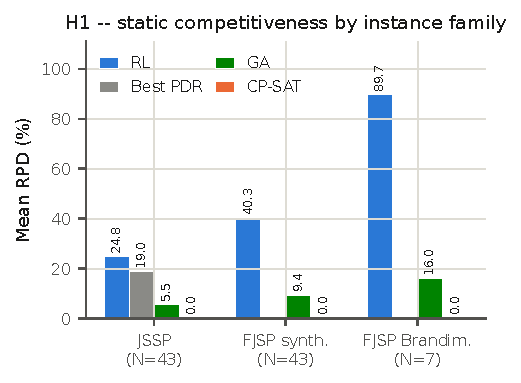
\includegraphics[width=0.62\textwidth]{figures/Fig_P1_h1_rpd_overview.pdf}
\caption{Mean relative percentage deviation (RPD) by method and instance family. RPD is computed against CP-SAT's makespan as the near-optimal reference within each family; the pre-registered H1 test itself compares the policy against the best PDR (JSSP) or the better of \{GA, CP-SAT\} (FJSP arms) on a per-instance basis (see text).}
\label{fig:h1}
\end{figure}

\begin{table}[htbp]
\centering
\caption{Mean and standard deviation of RPD (\%) by method, JSSP arm ($N=43$ instances, seed-0 deterministic evaluation).}
\label{tab:rpd-full}
\small
\begin{tabular}{llcc}
\toprule
\textbf{Method} & \textbf{Type} & \textbf{Mean RPD (\%)} & \textbf{SD (\%)} \\
\midrule
CP-SAT & Exact & 0.02 & 0.13 \\
GA & Metaheuristic & 5.52 & 5.31 \\
FIFO & PDR & 19.15 & 11.10 \\
RL (this study) & GNN--PPO policy & 24.82 & 12.92 \\
MOR & PDR & 39.83 & 16.91 \\
MWKR & PDR & 42.59 & 16.19 \\
SPT & PDR & 268.23 & 114.01 \\
LPT & PDR & 281.88 & 116.91 \\
EDD & PDR & 387.34 & 177.00 \\
LWKR & PDR & 391.91 & 177.61 \\
LOR & PDR & 401.15 & 174.56 \\
CR & PDR & 430.31 & 183.62 \\
\bottomrule
\end{tabular}
\end{table}

\clearpage
\subsection{H2 --- Size generalization (accepted)}
\label{sec:h2}

Across four size tiers ($1.5\times$--$3.0\times$ the training size, \emph{la21}--\emph{la40}), the Friedman test decisively rejects equal performance in each tier ($p<3.4\times10^{-6}$), and in every tier the policy's mean rank is not significantly different from the best PDR's ($\Delta$rank $0.20$--$1.00$ against a Nemenyi critical difference of $6.06$; Figure~\ref{fig:h2}). The critical-difference diagrams place the policy in the same statistically indistinguishable cluster as FIFO, MWKR, MOR, and SPT in all four tiers. This is an acceptance of \textbf{rank-relative, not absolute, competitiveness}: the policy's mean RPD (23.9--32.9\% across tiers) remains numerically above FIFO's (12.7--26.8\%) at every tier. The size--RPD relationship is non-monotonic: the $3.0\times$ tier has the lowest mean RPD of the four (23.86\%), below even the $1.5\times$ tier's (32.55\%)---a genuine, corroborated pattern rather than a sampling artifact, and one that cautions against assuming degradation is strictly monotonic in instance size for this architecture.

\begin{figure}[htbp]
\centering
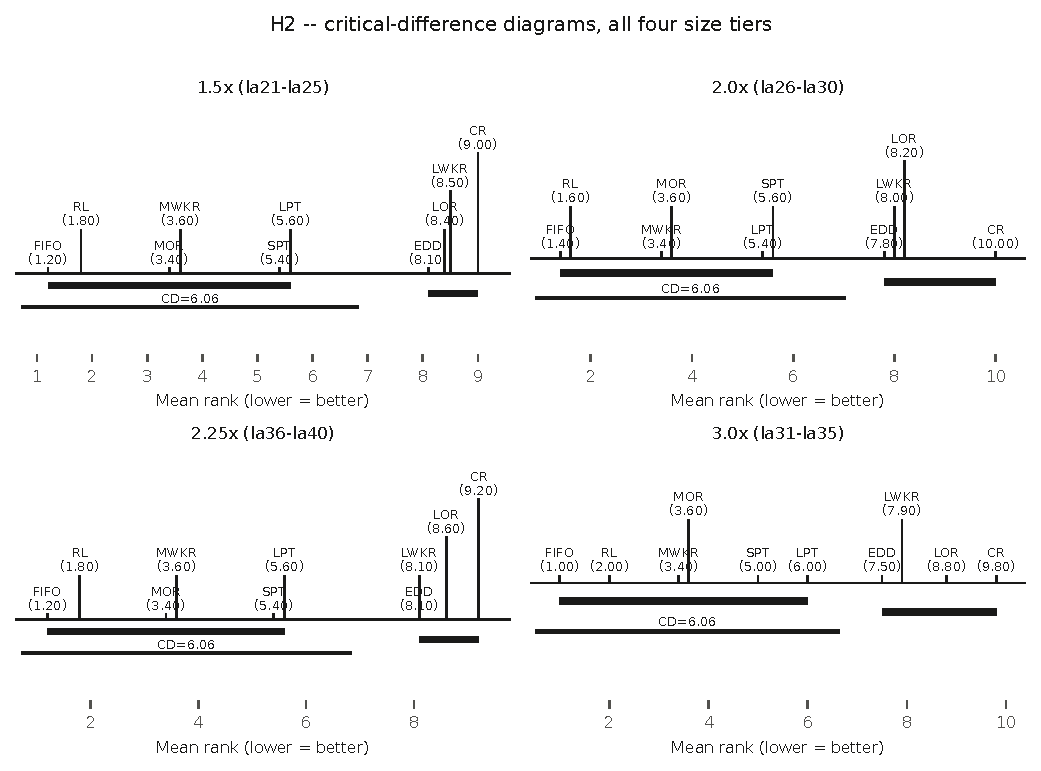
\includegraphics[width=0.92\textwidth]{figures/Fig_P2_h2_cd_grid.pdf}
\caption{Friedman--Nemenyi critical-difference diagrams for all four size tiers ($1.5\times$, $2.0\times$, $2.25\times$, $3.0\times$ the training size). Methods connected by a horizontal bar are not significantly different in mean rank (CD $=6.06$). The policy (RL) falls in the same top cluster as FIFO, MWKR, MOR, and SPT in every tier.}
\label{fig:h2}
\end{figure}

\subsection{H3/H4 --- Robustness and disruption-aware reward (rejected)}
\label{sec:h3h4}

The policy's robustness index (RI) is worse than the best PDR's in all nine disruption regimes, with large and uniformly consistent effect sizes ($r\approx-0.87$ in all nine; Figure~\ref{fig:h3}). The arrivals axis is the most severe (RI $\approx 1.65$--$1.82$ for the undisturbed, $\kappa{=}0$ policy, versus $0.26$--$0.28$ for the best PDR)---the axis furthest from the policy's training distribution, since dynamic arrivals present genuinely unseen mid-episode job insertions, whereas breakdowns and stochastic processing times only perturb the timing of operations the policy already expects to see. Extending the reward with the $\kappa\cdot\Delta_{\mathrm{inest}}$ instability penalty does not rescue robustness. At $\kappa=0.5$, all nine regimes show \emph{significantly worse} robustness, not better; at $\kappa=1.0$, only one of nine regimes improves significantly, short of the pre-registered five-of-nine threshold. Critically, both $\kappa$ values collapse nominal, undisturbed performance: nominal RPD increases by 106.0 percentage points at $\kappa=0.5$ and 46.6 percentage points at $\kappa=1.0$. We diagnose the likely root cause: both $\kappa{>}0$ policies were trained under domain-randomized sampling across all nine disruption regimes without ever including an undisturbed episode, which is sufficient on its own to explain the nominal collapse independent of whatever the $\Delta_{\mathrm{inest}}$ term itself contributes---a finding with direct, transferable implications for any attempt to extend single-disruption-type reward shaping \citep{zhang2024rewardshaping} to a multi-disruption training regime.

\begin{figure}[htbp]
\centering
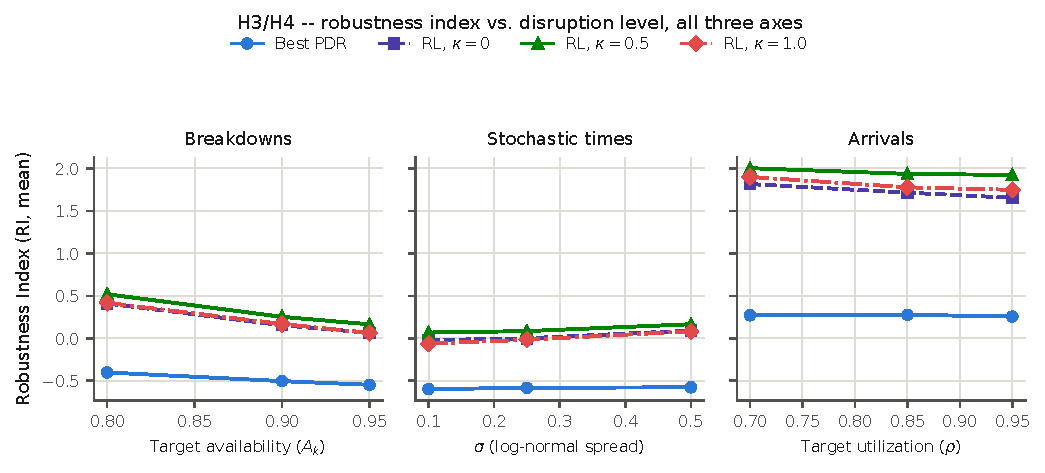
\includegraphics[width=0.98\textwidth]{figures/Fig_P3_h3h4_ri_combined.pdf}
\caption{Robustness index (RI, mean) versus disruption level, one panel per axis (breakdowns, stochastic processing times, arrivals). Lower RI is better. The best PDR (blue) remains well below all three RL variants ($\kappa=0,0.5,1.0$) on every axis and every level.}
\label{fig:h3}
\end{figure}

\clearpage
\subsection{H5 --- Decision latency (rejected under the strict threshold)}
\label{sec:h5}

The policy's per-decision latency is essentially flat across the full instance-size range---typically 4--11 ms, and never exceeding 44 ms even on the largest instances tested---while CP-SAT's total solve time is highly variable: near-instant on small, easy instances and saturating its 60-second budget on large or structurally hard ones (Figure~\ref{fig:h5}). Under the strict pre-registered criterion---the 1\% threshold must hold for \emph{every} instance---42 of 43 instances fail, driven largely by small instances where CP-SAT's near-instantaneous solve produces an artificially tiny per-decision denominator, a construct-validity limitation of dividing a one-shot solver's total solve time by operation count rather than evidence that the policy itself is slow. One large instance's CP-SAT measurement (\emph{la40}: 32{,}074 ms/decision, a $1{,}773\times$ ratio against the policy) was traced to a likely measurement anomaly via a raw-log audit; a sensitivity check substituting a structurally comparable instance's value (\emph{la38}, same 225-operation size class, both solved to a time-limited FEASIBLE result under the identical 60-second budget) reduces the ratio to $14.76\times$ but still rejects H5 under the strict threshold (Table~\ref{tab:la40})---the correction makes the rejection \emph{more}, not less, decisive, and is reported here precisely to make that transparent rather than to explain the result away. For genuinely large, hard instances that saturate CP-SAT's time budget, the policy retains a real one-to-two-order-of-magnitude latency advantage, a qualitative finding consistent with H5's motivating intuition even though the literal all-instances threshold is not met.

\begin{figure}[htbp]
\centering
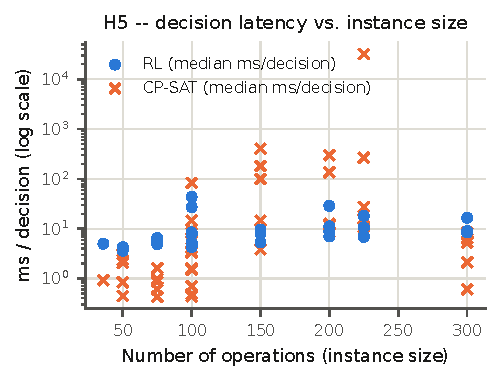
\includegraphics[width=0.62\textwidth]{figures/Fig_P4_h5_latency.pdf}
\caption{Per-decision latency (ms, log scale) versus instance size for the policy (RL) and CP-SAT. The policy's latency is essentially flat; CP-SAT's grows erratically with instance size and structural hardness.}
\label{fig:h5}
\end{figure}

\begin{table}[htbp]
\centering
\caption{Sensitivity check for the \emph{la40} CP-SAT latency measurement, substituting \emph{la38}'s wall-clock time (same size class, same FEASIBLE status under the identical 60\,s budget).}
\label{tab:la40}
\small
\begin{tabular}{lcccc}
\toprule
\textbf{Reading} & \textbf{RL (ms/dec.)} & \textbf{CP-SAT (ms/dec.)} & \textbf{Ratio} & \textbf{H5 passes (of 43)} \\
\midrule
Raw (as measured) & 18.09 & 32{,}074.09 & $1{,}773.5\times$ & 1 \\
Sensitivity-corrected (\emph{la38} subst.) & 18.09 & 266.91 & $14.8\times$ & 0 \\
\bottomrule
\end{tabular}
\end{table}

% ============================================================================
\section{Discussion}
\label{sec:discussion}
% ============================================================================

\subsection{Positioning against prior work}

\textbf{Relative to L2D.} The comparator used for H1 (the minimum RPD across nine PDRs, evaluated per instance) is intrinsically harder to beat than L2D's three fixed rules (SPT, MWKR, MOPNR)---FIFO, the dominant rule for the large majority of instances evaluated here, is not among L2D's comparators---so the raw win-rate figures (18.6\% here versus L2D's 87.5--92\%) are not directly comparable across studies. Training budget likely also differs by orders of magnitude, though \citet{zhang2020l2d} do not report a figure that would allow a verified comparison. H1's rejection is best read as ``this instantiation, under this training budget, is not competitive,'' not as a categorical claim about the relational-GIN architecture.

\textbf{Relative to L2D and SPM-DAN on generalization.} L2D's own generalization gap (9.4\% at $4$--$5\times$ training size) stays far below the best PDR's gap at that size (33.7--54.9\%)---the same qualitative pattern observed here---but starting from a far more competitive base policy, so L2D's generalization preserves absolute competitiveness where the present result preserves only rank. This is consistent with, and illustrates cleanly, a reading of GNN generalization theory \citep{xu2019gin} in which size-invariance is a \emph{multiplicative} property acting on whatever competitiveness the base policy already has, rather than a mechanism that improves it outright. SPM-DAN \citep{smit2025spmdan} generalizes far more strongly in absolute terms ($-7.10\%$ versus $23.9$--$32.9\%$ here) but under a single uncertainty source and with a scenario-processing module purpose-built for that axis---suggestive evidence that a dedicated architectural mechanism for the specific uncertainty axis being generalized outperforms a generic relational encoder without one.

\textbf{H3/H4 as the first joint test of the generalization--robustness combination.} \citet{lassoued2026} show that a plain maskable-PPO policy can outperform dispatching rules under combined breakdown-and-arrival disruption when robustness is the only training objective, with no size-generalization requirement sharing the same architecture and training budget. The policy evaluated here, pursuing both objectives simultaneously, loses decisively to the same class of dispatching rules under disruption. Read together, this is, to our knowledge, the first quantitative evidence that the joint objective is not free: a policy whose capacity and training regime are spent entirely on one axis can beat dispatching rules on that axis; a policy splitting the same budget across two axes loses decisively on the robustness axis. This does not prove the joint objective is unattainable in principle---no architectural ablation isolating the relational encoder's specific contribution to each axis was run in this study---but it is, to our knowledge, the first controlled demonstration that the tension between the two objectives is real and measurable rather than merely assumed. The mechanism diagnosed for H4 (domain-randomized training without nominal-episode exposure) is itself a transferable caution for the broader disruption-aware reward-shaping literature \citep{zhang2024rewardshaping}, which has not previously needed to confront a multi-disruption training regime.

\subsection{The central finding: generalization and robustness as separable properties}

Taken together, the pattern across H1--H5 supports a specific, falsifiable reading of GNN--PPO scheduling policies: size-invariant architecture (Section~\ref{sec:architecture}) transfers rank-relative competitiveness---H2 is accepted even though the underlying policy is, by H1, not itself competitive in absolute terms---while robustness to disruption does not emerge as a free byproduct of that same architecture (H3 rejected) and cannot be induced by a na\"ively multi-disruption-trained reward term without an unacceptable competitiveness cost (H4 rejected, with a diagnosed cause). We hold this pattern, rather than any single accepted or rejected hypothesis in isolation, as the study's central and most defensible contribution. It does not depend on the policy ``winning'' any individual comparison, and is therefore not undermined by the fact that it loses to PDR and GA baselines on most measures; that loss is part of the finding, not a threat to it. It is grounded in a pre-registration timestamp and frozen decision rules, which pre-empts the most common concern raised against negative-result reinforcement-learning studies---that hypotheses or thresholds were adjusted after seeing the data. And it directly answers the specific, citable gap identified in Section~\ref{sec:gap}: no prior work identified in our review jointly tests size generalization and multi-disruption robustness for a GNN--PPO scheduling policy under one statistically powered protocol.

\subsection{Threats to validity and limitations}

Several limitations qualify these conclusions. A single training seed per $\kappa$ condition limits the precision, though not necessarily the direction, of the H4 magnitudes; multi-seed replication is identified as priority future work. A structural asymmetry between the $\kappa{=}0$ condition (a statically trained policy evaluated through an adapter against the dynamic environment) and the $\kappa{>}0$ conditions (trained natively against the dynamic contract) means $\Delta \RI$ is not a fully clean isolation of the reward term's effect from this training-regime difference. All evaluation is simulation-only, using three parametric disruption generators (exponential/log-normal breakdowns, log-normal processing-time noise, Poisson arrivals) whose fidelity to disruption processes on a real shop floor is assumed from the wider simulation literature \citep{law2024,sargent2011} rather than validated against field data; any claim about deployability should be read strictly within this simulation-only scope. Finally, H3's rejection is diagnosed in this study primarily through the arrivals axis being furthest from the training distribution, but the present design does not include an architectural ablation that would isolate the relational encoder's specific contribution to robustness from the training regime's contribution---a natural next step, discussed below.

\subsection{Theoretical and practical implications}

Theoretically, the H1/H2 contrast offers a clean empirical illustration that size-invariant architecture and base-policy competitiveness are separable design axes: an architecture can be permutation-invariant enough to preserve relative rank under scale-up while remaining, in absolute terms, an uncompetitive policy---consistent with a multiplicative reading of GNN generalization theory in which the architecture transfers whatever competitiveness the base policy already has, rather than manufacturing competitiveness on its own. The H3/H4 result extends this logic to a second axis: robustness to disruption is not a passive byproduct of a size-invariant encoder, and a reward term explicitly designed to induce it can fail not because the term is wrong in principle, but because of an identifiable interaction with the training regime around it (domain randomization without nominal exposure). Both findings argue for treating generalization, robustness, and reward design as separable axes to be evaluated and engineered independently, rather than assuming that solving one implies progress on the others---a methodological caution directly relevant to the growing body of GNN-based scheduling research surveyed in Section~\ref{sec:litrev}.

Practically, the contrast between H1/H3's quality weakness and H5's qualitative speed strength motivates, without itself fully evaluating, a hybrid deployment pattern for real scheduling systems: a fast reactive policy could serve as an immediate decision bridge in the seconds following a disruption event, while an exact or metaheuristic re-optimizer computes a higher-quality replacement schedule in parallel---assigning each method the role its own results in this study actually support (the policy as a fast, immediately available fallback; CP-SAT or the GA as the quality-of-solution engine), rather than requiring a single method to be simultaneously the fastest and the best. For practitioners evaluating GNN--DRL scheduling tools, the results also caution against inferring disruption robustness from a size-generalization claim alone: this study's own evidence is that the two do not co-occur automatically, and each should be requested and verified as a separate, explicitly tested capability.

% ============================================================================
\section{Conclusion}
\label{sec:conclusion}
% ============================================================================

This study pre-registered and tested five hypotheses about whether a relational-GIN, PPO-based scheduling policy can jointly generalize across instance sizes and remain robust to multiple simultaneous disruption types in the dynamic, stochastic flexible job-shop problem. Four of five hypotheses are rejected, one is accepted, and, critically, every rejection is diagnosed to a concrete, actionable mechanism rather than left as an unexplained negative result: the arrivals axis being furthest from the training distribution for H3, a domain-randomized training regime that never exposes the policy to undisturbed operation for H4, and a per-decision latency metric with a construct-validity weakness for one-shot solvers for H5. The accepted hypothesis, H2, demonstrates that size-invariant architecture transfers rank-relative competitiveness even from a base policy that is not itself competitive in absolute terms---direct empirical support for permutation-invariance-based GNN generalization theory, independent of the underlying policy's absolute strength. Taken together, we hold this pattern---architectural transfer of one property, no automatic transfer of the other, with a diagnosed and actionable cause for the gap in every case---as the study's central, defensible contribution: to our knowledge, the first statistically rigorous, pre-registered evidence that size generalization and multi-disruption robustness are separable properties of GNN--PPO scheduling policies, not a package deal. Future work includes an architectural ablation isolating the relational encoder's specific contribution to each axis independently of training regime; a corrected domain-randomization training procedure that preserves nominal-episode exposure; multi-seed replication of the $\kappa$ ablation to sharpen the precision of the H4 magnitudes; and, ultimately, validation against disruption data from a real production environment, since every result reported here is obtained under simulation.

\paragraph{Data availability statement.} The simulation environment, policy implementation, trained checkpoints, and the complete experimental results and analysis code supporting the findings of this study are maintained in a version-controlled repository, with a permanent archival deposit in preparation at the time of writing. Repository and deposit identifiers will be provided upon acceptance; interested readers may contact the corresponding author in the interim.

\paragraph{Funding.} This research did not receive any specific grant from funding agencies in the public, commercial, or not-for-profit sectors.

\paragraph{Declaration of competing interest.} The author declares no known competing financial interests or personal relationships that could have appeared to influence the work reported in this article.

\bibliography{references}

\end{document}
